\section{Taratura di una sonda a filo caldo}
La presente esercitazione si pone come obiettivo la taratura di una sonda a filo caldo da strato limite Dantec P15. La finalità è definire l'equazione di taratura nella forma prevista dalla legge di King e nella forma polinomiale.
\begin{figure}[H]
    \centering
    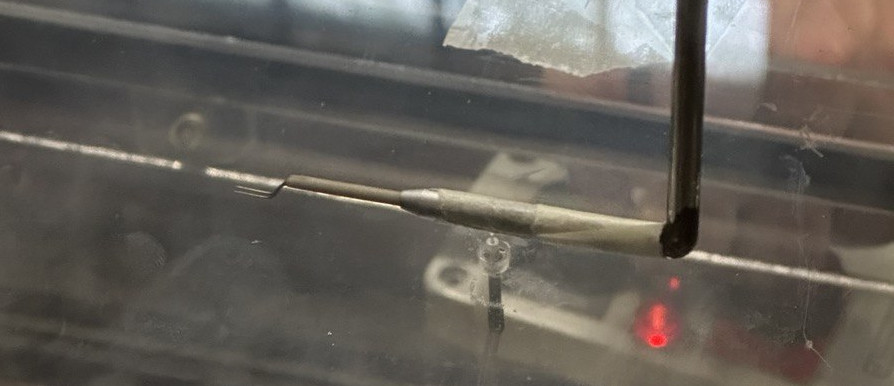
\includegraphics[width=.8\textwidth]{images/8/sondahw.jpg}
    \caption{Sonda a filo caldo da strato limite Dantec P15}
\end{figure}

\subsection{Descrizione dell'esperimento}
L'anemometria è lo studio dei metodi e delle tecniche necessarie per la misura di velocità nei flussi. In particolare, l'anemometria a filo caldo si basa sullo scambio termico convettivo tra un elemento sensibile riscaldato e il flusso che lo investe, del quale si vuole misurare la velocità istantanea. Le sonde a filo caldo hanno una bassissima intrusività ed un'elevata risposta in frequenza (si arriva fino alle centinaia di kHz), queste due caratteristiche rendono la tecnica dell'anemometria a filo caldo adatta a misure di velocità dei flussi turbolenti.\\\\
L'anemometria a filo caldo non è una tecnica assoluta, pertanto la sonda necessita di taratura. Una sonda a filo caldo necessita di taratura anche diverse volte nel corso di una giornata, questo perché la curva di taratura è dipendente dalla temperatura.\\\\
L'elemento sensibile di un anemometro a filo caldo consiste in un filo metallico di diametro estremamente piccolo ($d=5\mu m$), di lunghezza dell'ordine del millimetro, mantenuto caldo per effetto Joule dall'attraversamento di una corrente elettrica.\\\\
Il sensore caldo (hot wire) ad una certa temperatura superiore a quella del fluido viene raffreddato dalla corrente che lo investe provocando una variazione di temperatura del sensore e conseguentemente una variazione della resistenza elettrica del sensore stesso. Ad una variazione di velocità corrisponde quindi una differenza di potenziale ai capi di una diagonale di un ponte di Wheatstone, di cui la sonda fa parte come uno dei quattro rami.\\\\
Si consideri un elemento cilindrico metallico infinitamente lungo, percorso da corrente elettrica ed immerso in un flusso gassoso uniforme. La quantità di calore scambiata tra il filo e la corrente fluida dipende da:
\begin{itemize}
    \item Velocità della corrente $U$;
    \item Differenza di temperatura tra sensore e fluido $T_w-T_f$;
    \item Proprietà del fluido: $\rho$, $\mu$, $k_f$, $c_p$;
    \item Proprietà del filo sensore (coefficienti di resistività $b$);
    \item Dimensioni del sensore: $l$ e $d$;
    \item Direzione della corrente: $\alpha$.
\end{itemize}
Lo scambio termico avviene per effetto di convezione forzata $q_f$, convezione naturale $q_n$, conducibilità dal filo verso i supporti metallici $q_c$ ed irraggiamento verso l'esterno $q_i$. Lo scambio termico dominante è rappresentato dalla convezione forzata.\\\\
Per un filo di lunghezza $l$ e diametro $d$, la quantità di calore $q$ trasferita nell'unità di tempo dal filo caldo alla corrente fluida a temperatura più bassa è data da:
\begin{equation*}
    q = h(\pi d l) (T_w - T_f)
\end{equation*}
Dove $h$ è il coefficiente di scambio termico per convezione forzata.\\\\
In condizioni di equilibrio termico il calore scambiato tra sensore e corrente fluida è bilanciato da quello generato nell'unità di tempo per effetto Joule dalla corrente elettrica che attraversa il filo:
\begin{equation*}
    q_J = R_w I^2
\end{equation*}
Risulta quindi il bilancio di scambio termico:
\begin{equation*}
    I^2R_w = h\pi d l (T_w - T_f)
\end{equation*}
La dipendenza del flusso di calore scambiato dalla velocità è racchiuso nel coefficiente di scambio termico $h$. Ricorrendo all'analisi dimensionale e all'applicazine del teorema di Buckingham, il coefficiente $h$ può essere espresso attraverso il numero di Nusselt:
\begin{equation*}
    Nu = \frac{ h d}{k_f} \quad \rightarrow \quad h = \frac{Nu\, k_f}d
\end{equation*}
Sostituendo l'equazione del numero di Nusselt nel bilancio termico si ottiene:
\begin{equation*}
    R_w I^2 = \pi l k_f (T_w - T_f) Nu
\end{equation*}
L'analisi dimensionale comporta che il numero di Nusselt dipende da:
\begin{equation*}
    Nu = f(Re, Pr, M, Gr, Kn, T_w-T_f, l/d, \alpha)
\end{equation*}
Dove compaiono i vari numeri adimensionali rappresentativi di specifiche fenomenologie: il numero di Reynolds $Re$, il numero di Prandtl $Pr$, il numero di Grashof $Gr$, il numero di Mach $M$, il numero di Knudsen $Kn$... Questa relazione però è molto complessa per usi pratici e si procede pertanto con una semplificazione.\\\\
Il parametro dominante risulta essere il numero di Reynolds nel caso di flussi incomprimibili, in quanto lo scambio termico corrente-cilindro dipende fortemente dalla configurazione del campo di moto nello strato limite del cilindro che cambia profondamente in funzione del numero di Reynolds.\\\\
Considerando la sola convezione forzata ed il filo infinitamente lungo, sono state proposte diverse leggi di scambio termico o di raffreddamento in forma adimensionale. Una di queste è la legge di King:
\begin{equation*}
    Nu = 1 +\sqrt{2\pi Pr Re}
\end{equation*}
È importante notare come secondo questa legge $Nu\propto \sqrt{Re}$, ovvero $h\propto U^{1/2}$.\\\\
Si riconsideri l'equazione di bilancio termico:
\begin{equation*}
    I^2 R_w = \pi l k_f (T_w - T_f) Nu
\end{equation*}
La dipendenza della resistenza del sensore $R_w$ dalla temperatura produce un altro effetto su cui si basa il funzionamento di un anemometro a filo caldo. Tale dipendenza funzionale può essere espressa dalla relazione:
\begin{equation*}
    R_w = R_0 [1 + f(T_w, T_0, b)]
\end{equation*}
Dove $R_0$ è la resistenza alla temperatura di riferimento $T_0$ e che può anche coincidere con la resistenza $R_f$ calcolata alla temperatura del fluido $T_f$. Per le usuali temperature di operazione i termini non lineari si possono trascurare, pertanto si ottiene:
\begin{equation*}
    R_w = R_f[1+b(T_w-T_f)]
\end{equation*}
Il salto di temperatura si esprime quindi come:
\begin{equation*}
    T_w - T_f = \frac{R_w - R_f}{bR_f}
\end{equation*}
Sostituendo nel bilancio termico si ottiene:
\begin{equation*}
    I^2 R_w = \pi l k_f Nu \frac{R_w - R_f}{bR_f}
\end{equation*}
Considerando la relazione di Kramers, secondo cui:
\begin{equation*}
    Nu = 0.42 Pr^{0.2} + 0.57 Pr^{0.33} Re^{0.5}
\end{equation*}
Si ottiene:
\begin{equation*}
    I^2R_w = \frac{\pi l k_f}b \frac{R_w - R_f}{R_f} [0.42 Pr^{0.2} + 0.57 Pr^{0.33} Re^{0.5}]
\end{equation*}
Questa relazione, per l'applicazione anemometrica, è conveniente scriverla nella forma:
\begin{equation*}
    \frac{I^2R_w}{R_w-R_f} = A + B \sqrt{Re}
\end{equation*}
Nel caso reale, dove è presente una lunghezza finita del sensore, la relazione assume la stessa scrittura ma le costanti $A$ e $B$ vanno determinate sperimentalmente.\\\\
Per un dato fluido e un dato sensore in generale si opera con una relazione semplificata del tipo:
\begin{equation*}
    \frac{E^2}{R_w^2}\frac{R_w}{R_w-R_f} = A + B U^n
\end{equation*}
Sono stati sviluppati due diversi sistemi anemometrici:
\begin{itemize}
    \item Corrente costante $I_w=cost$;
    \item Temperatura costante $T_w=cost$.
\end{itemize}
Per un sistema a temperatura costante, se anche la temperatura del fluido rimane costante, ne risulta che $R_w$ è costante. Pertanto, si ottiene un legame diretto tra $E^2$ e $U^n$ attraverso le costanti $A$ e $B$:
\begin{equation*}
    E^2 = A + B U^n
\end{equation*}
Questa relazione prende il nome di Legge di King.

\subsection{Catena di misura}
Per la presente attività, la taratura viene effettuata in situ, la sonda a filo caldo da strato limite è quindi posizionata nella camera di prova di una galleria del vento aperta. Per la misura della velocità della corrente si utilizza un tubo di Pitot accoppiato con il trasduttore di pressione differenziale Setra 239 C già tarato. Il sistema anemometrico è Dantec Dynamics.\\\\
La catena di misura è quindi composta da:
\begin{itemize}
    \item Galleria del vento aperta;
    \item Sonda a filo caldo da strato limite Dantec P15;
    \item Ponte di Wheatsone e circuito di condizionamento;
    \item Tubo di Pitot;
    \item Trasduttore di pressione Setra 239 C;
    \item Sistema di acquisizione dati e PC con LabView.
\end{itemize}

\newpage
\subsection{Procedura sperimentale}
Come primo passo si misurano la pressione e la temperatura ambiente, dalle quali si ricava la densità utilizzando la legge dei gas perfetti e la viscosità dinamica utilizzando la legge di Sutherland:
\begin{equation*}
    \rho = \frac{p_{amb}}{RT_{amb}} \qquad \mu = 1.46\cdot10^{-6} \frac{T_{amb}^{3/2}}{T_{amb}+110} 
\end{equation*}
Successivamente è necessario bilanciare il ponte di Wheatstone della sonda. La tensione di bilanciamento deve essere tale da avere una differenza di potenziale nulla ai capi della sonda a filo caldo.\\\\
Per ogni velocità $U$ del flusso in galleria del vento, una volta esauriti eventuali fenomeni transitori, sono effettuate due letture: una per il segnale di tensione in uscita dalla sonda filo caldo $E_{HW}$ ed un'altra relativa al segnale di tensione in uscita dal trasduttore di pressione collegato al tubo di Pitot $E_t$.\\\\
La sonda a filo caldo lavora a temperatura costante ed è posta perpendicolarmente alla corrente, si parla quindi di taratura in velocità (angoli $\alpha$ e $\beta$ nulli).\\\\
I dati grezzi misurati con la procedura appena descritta sono riportati nelle tabelle in appendice \ref{a8}.

\subsection{Analisi dati}
L'analisi dati per la presente attività è condotta con l'ausilio di un codice Python, riportato in appendice \ref{b8}.\\\\
Come prima operazione è necessario misurare la tensione di offset del trasduttore di pressione Setra 239 C. Tale tensione per la presente indagine risulta essere pari a $E_{0t}=0.036$ V.\\\\
Utilizzando la costante di taratura del trasduttore di pressione precedentemente ricavata:
\begin{equation*}
    K_t =\ 550 \text{Pa/m}
\end{equation*}
Si misura la pressione dinamica e quindi la velocità del flusso rilevata dal tubo di Pitot:
\begin{equation*}
    U_{pitot} = \sqrt{\frac{2K_t(E_{t}-E_{0t})}\rho}
\end{equation*}
Diagrammando la tensione in uscita della sonda a filo caldo in funzione della velocità del flusso per le quattro squadre si ottiene il seguente diagramma:
\begin{figure}[H]
    \centering
    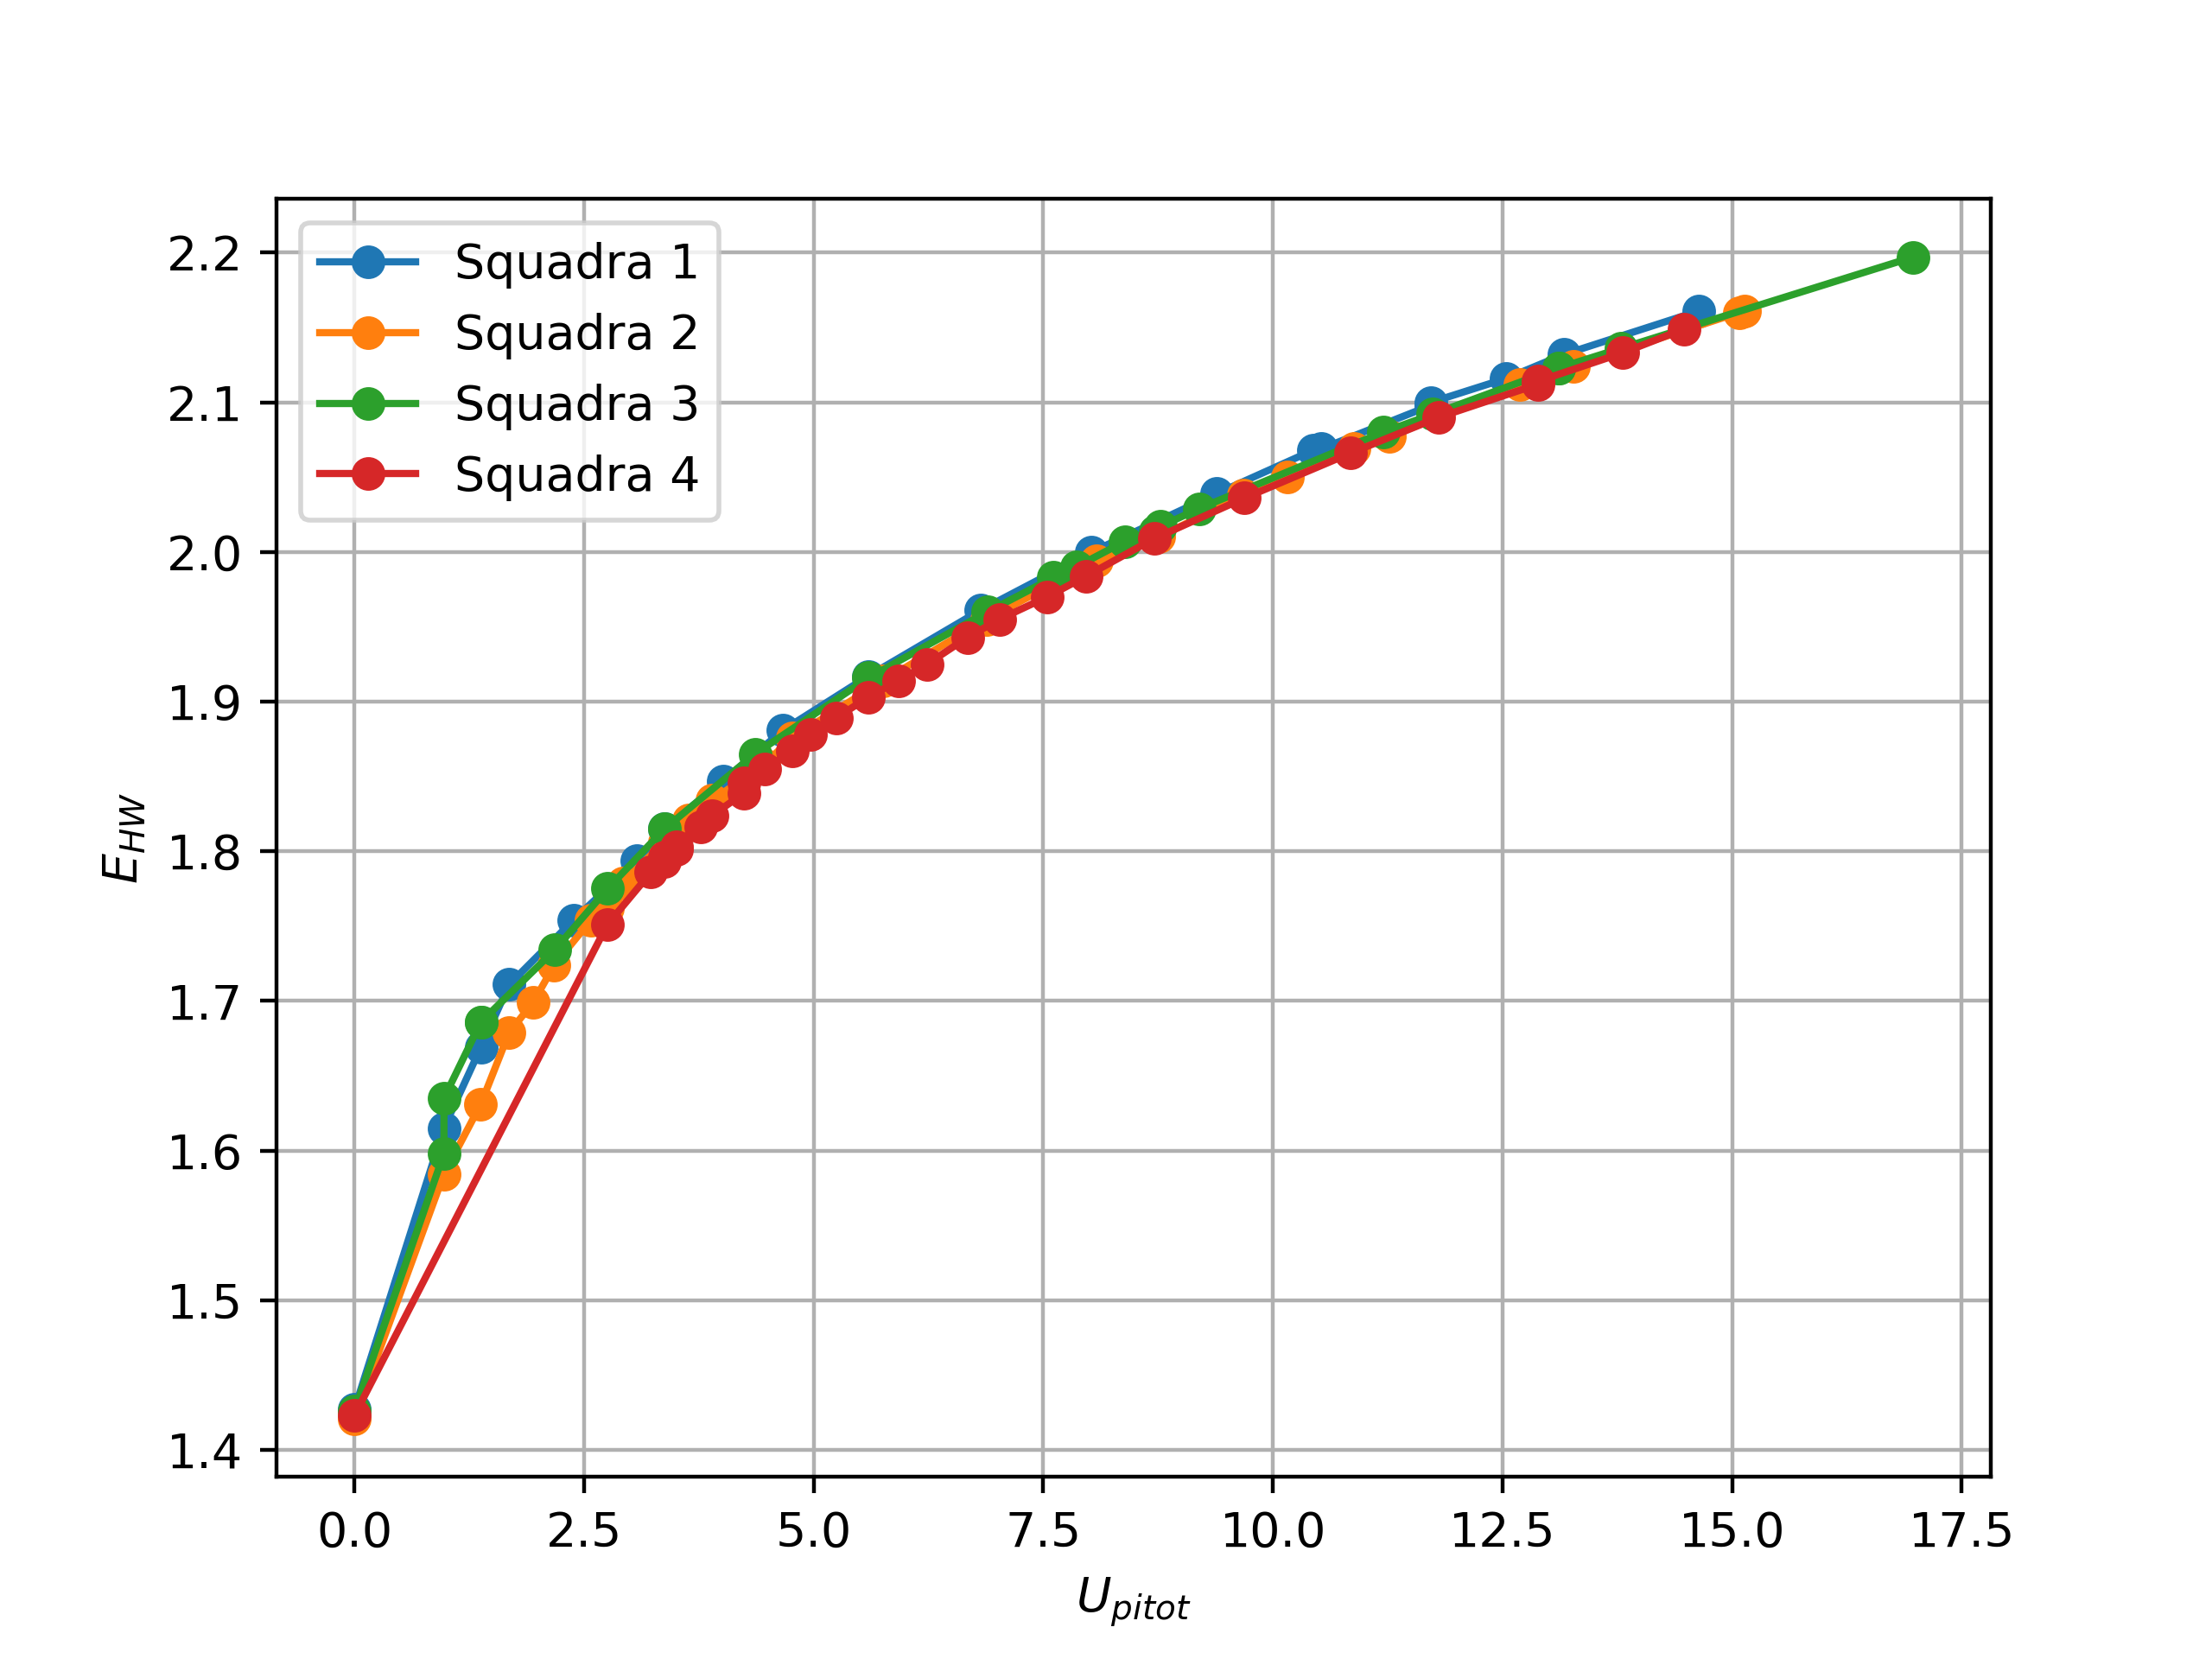
\includegraphics[width=.8\textwidth]{images/8/rawdata.png}
    \caption{Dati di taratura $E_{HW}=f(U_{Pitot})$}
\end{figure}

\noindent Si vogliono ora ricavare i coefficienti $A$, $B$ e $n$ della legge di King:
\begin{equation*}
    E^2 = A + BU^n
\end{equation*}
Per quanto riguarda il coefficiente $A$, si nota immediatamente che quando la velocità del flusso è nulla ($U=0$), tale coefficiente coincide con la tensione di offset al quadrato:
\begin{equation*}
    A = E_0^2
\end{equation*}
Si può scrivere quindi:
\begin{equation*}
    E^2 - E_0^2 = BU^n
\end{equation*}
Rimaneggiando tale relazione utilizzando i logaritmi si ottiene l'equazione di una retta:
\begin{equation*}
    \ln(E^2-E_0^2) = \ln B + n \ln U \quad \rightarrow \quad y = c + kx
\end{equation*}
Pertanto, interpolando linearmente i dati, si ricavano i valori delle costanti $B$ ed $n$. Per le quattro squadre, questi valori sono:\\\\
\textbf{Legge di King}
\begin{equation*}
    \begin{split}
        \text{Squadra 1}\quad& A = 2.036 \quad B = 0.638 \quad n = 0.536\\
        \text{Squadra 2}\quad& A = 2.019 \quad B = 0.587 \quad n = 0.572\\
        \text{Squadra 3}\quad& A = 2.033 \quad B = 0.639 \quad n = 0.532\\
        \text{Squadra 4}\quad& A = 2.025 \quad B = 0.628 \quad n = 0.535
    \end{split}
\end{equation*}
Una volta ottenuta la legge di King, si può ricavare il valore di velocità relativa ad un certo valore di tensione della sonda a filo caldo $E$ mediante la seguente relazione:
\begin{equation*}
    U_{K} = \left( \frac{E^2 - A}{B} \right)^{1/n}
\end{equation*}
Per quanto riguarda le equazioni polinomiali, queste si scrivono, per una generica legge di grado $n$, come:
\begin{equation*}
    U_{n} = a_0 + a_1 E + a_2 E^2 + ... + a_n E^n
\end{equation*}
Pertanto, mediante una semplice interpolazione polinomiale dei dati sperimentali, è possibile ricavare gli $n+1$ coefficienti $a_i$. In particolare, si ricavano tali coefficienti per le leggi polinomiali di terzo, quarto e quinto grado:\\\\

\textbf{Legge polinomiale di terzo grado}
\begin{table}[H]
    \centering
    \begin{tabular}{|c|c|c|c|c|}
    \hline
              & $a_0$    & $a_1$    & $a_2$     & $a_3$   \\ \hline
    Squadra 1 & -59.9903 & 129.2135 & -94.6522  & 23.5231 \\ \hline
    Squadra 2 & -89.0844 & 179.5354 & -123.3823 & 28.9793 \\ \hline
    Squadra 3 & -61.6043 & 134.0607 & -98.7698  & 24.5912 \\ \hline
    Squadra 4 & -80.2433 & 162.0433 & -112.2028 & 26.6750 \\ \hline
    \end{tabular}
\end{table}

\textbf{Legge polinomiale di quarto grado}
\begin{table}[H]
    \centering
    \begin{tabular}{|c|c|c|c|c|c|}
    \hline
              & $a_0$     & $a_1$    & $a_2$     & $a_3$    & $a_4$    \\ \hline
    Squadra 1 & -87.2494  & 190.9173 & -146.6365 & 42.8496  & -2.6763  \\ \hline
    Squadra 2 & -332.8080 & 731.1313 & -588.0082 & 201.6790 & -23.9084 \\ \hline
    Squadra 3 & -126.9414 & 281.1389 & -221.9210 & 70.0656  & -6.2504  \\ \hline
    Squadra 4 & -397.9412 & 872.7634 & -703.5834 & 243.7801 & -29.6903 \\ \hline
    \end{tabular}
\end{table}

\textbf{Legge polinomiale di quinto grado}
\begin{table}[H]
    \centering
    \begin{tabular}{|c|c|c|c|c|c|c|}
    \hline
              & $a_0$    & $a_1$   & $a_2$    & $a_3$   & $a_4$    & $a_5$  \\ \hline
    Squadra 1 & -1631.30 & 4522.25 & -4979.79 & 2725.06 & -743.13  & 81.36  \\ \hline
    Squadra 2 & -1240.07 & 3289.56 & -3457.69 & 1802.33 & -467.96  & 49.03  \\ \hline
    Squadra 3 & -1736.09 & 4776.18 & -5215.03 & 2827.52 & -763.50  & 82.74  \\ \hline
    Squadra 4 & -3110.52 & 8338.70 & -8877.45 & 4695.51 & -1236.28 & 130.24 \\ \hline
    \end{tabular}
\end{table}

\newpage
\noindent Diagrammando l'andamento della legge di King e delle tre leggi polinomiali ottenute, assieme ai valori sperimentali, si ottengono i seguenti diagrammi per le quattro squadre:
\begin{figure}[H]
    \centering
    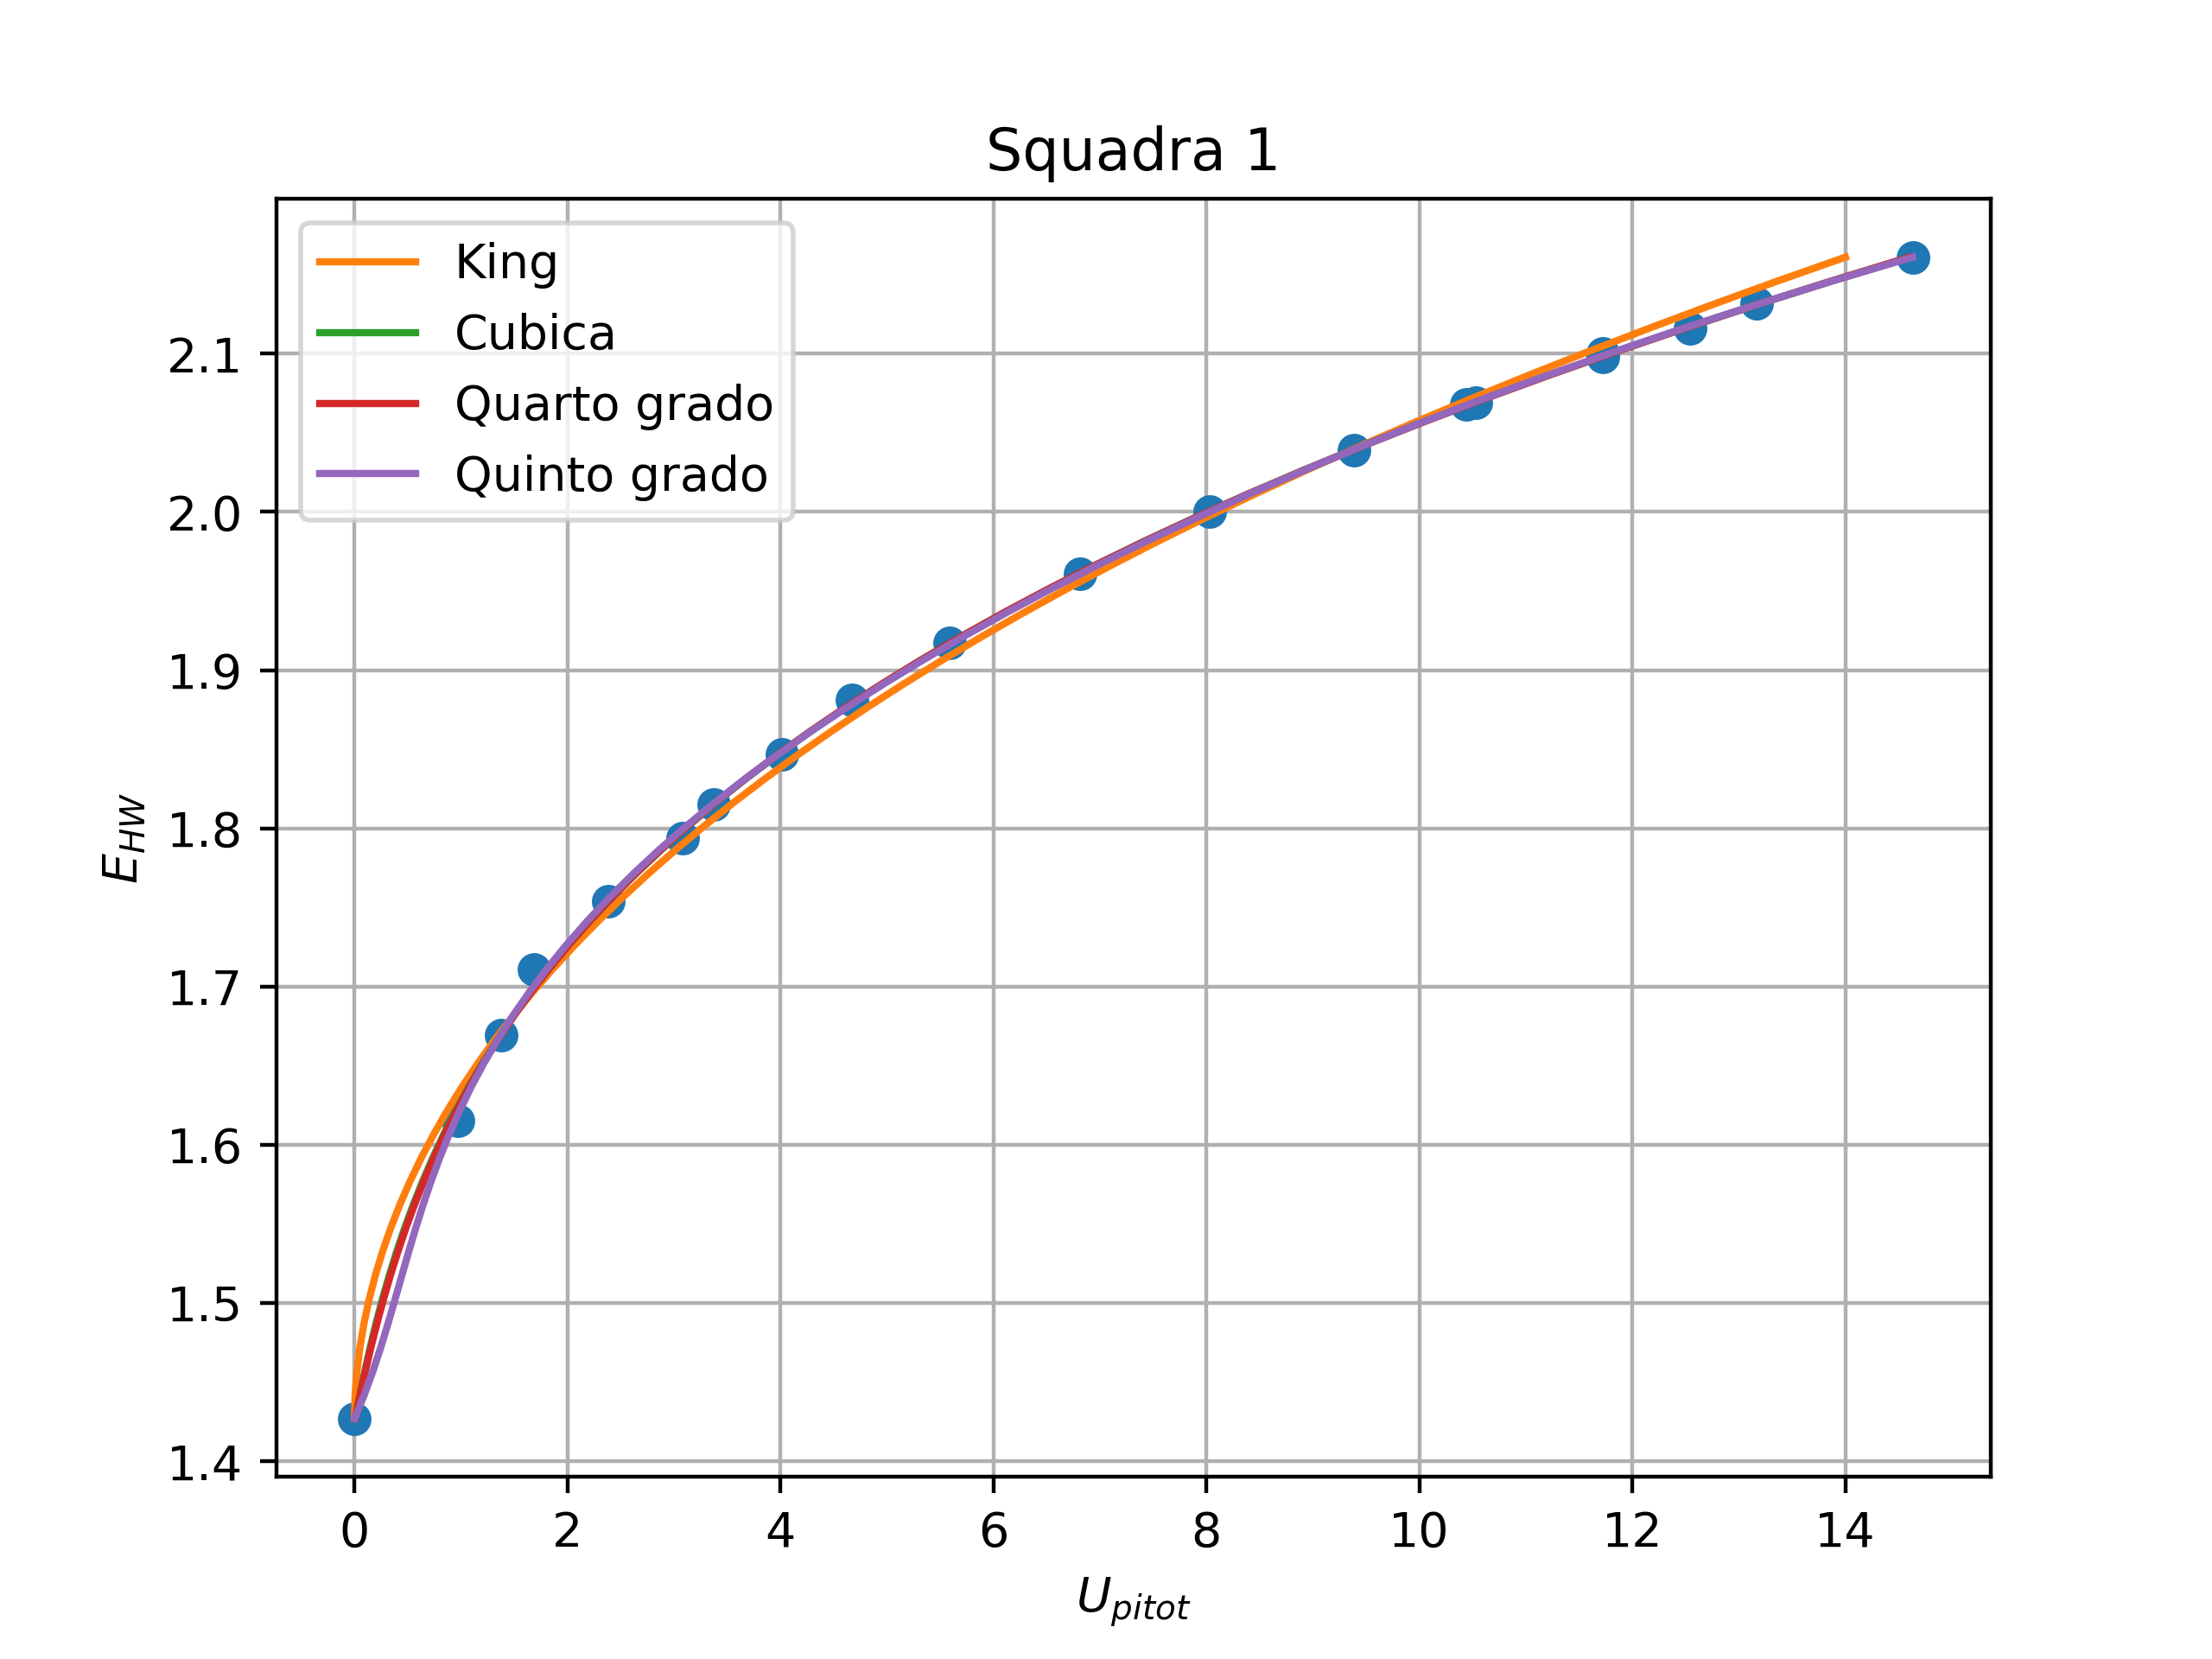
\includegraphics[width=.8\textwidth]{images/8/sq1.png}
    \caption{Squadra 1}
\end{figure}
\begin{figure}[H]
    \centering
    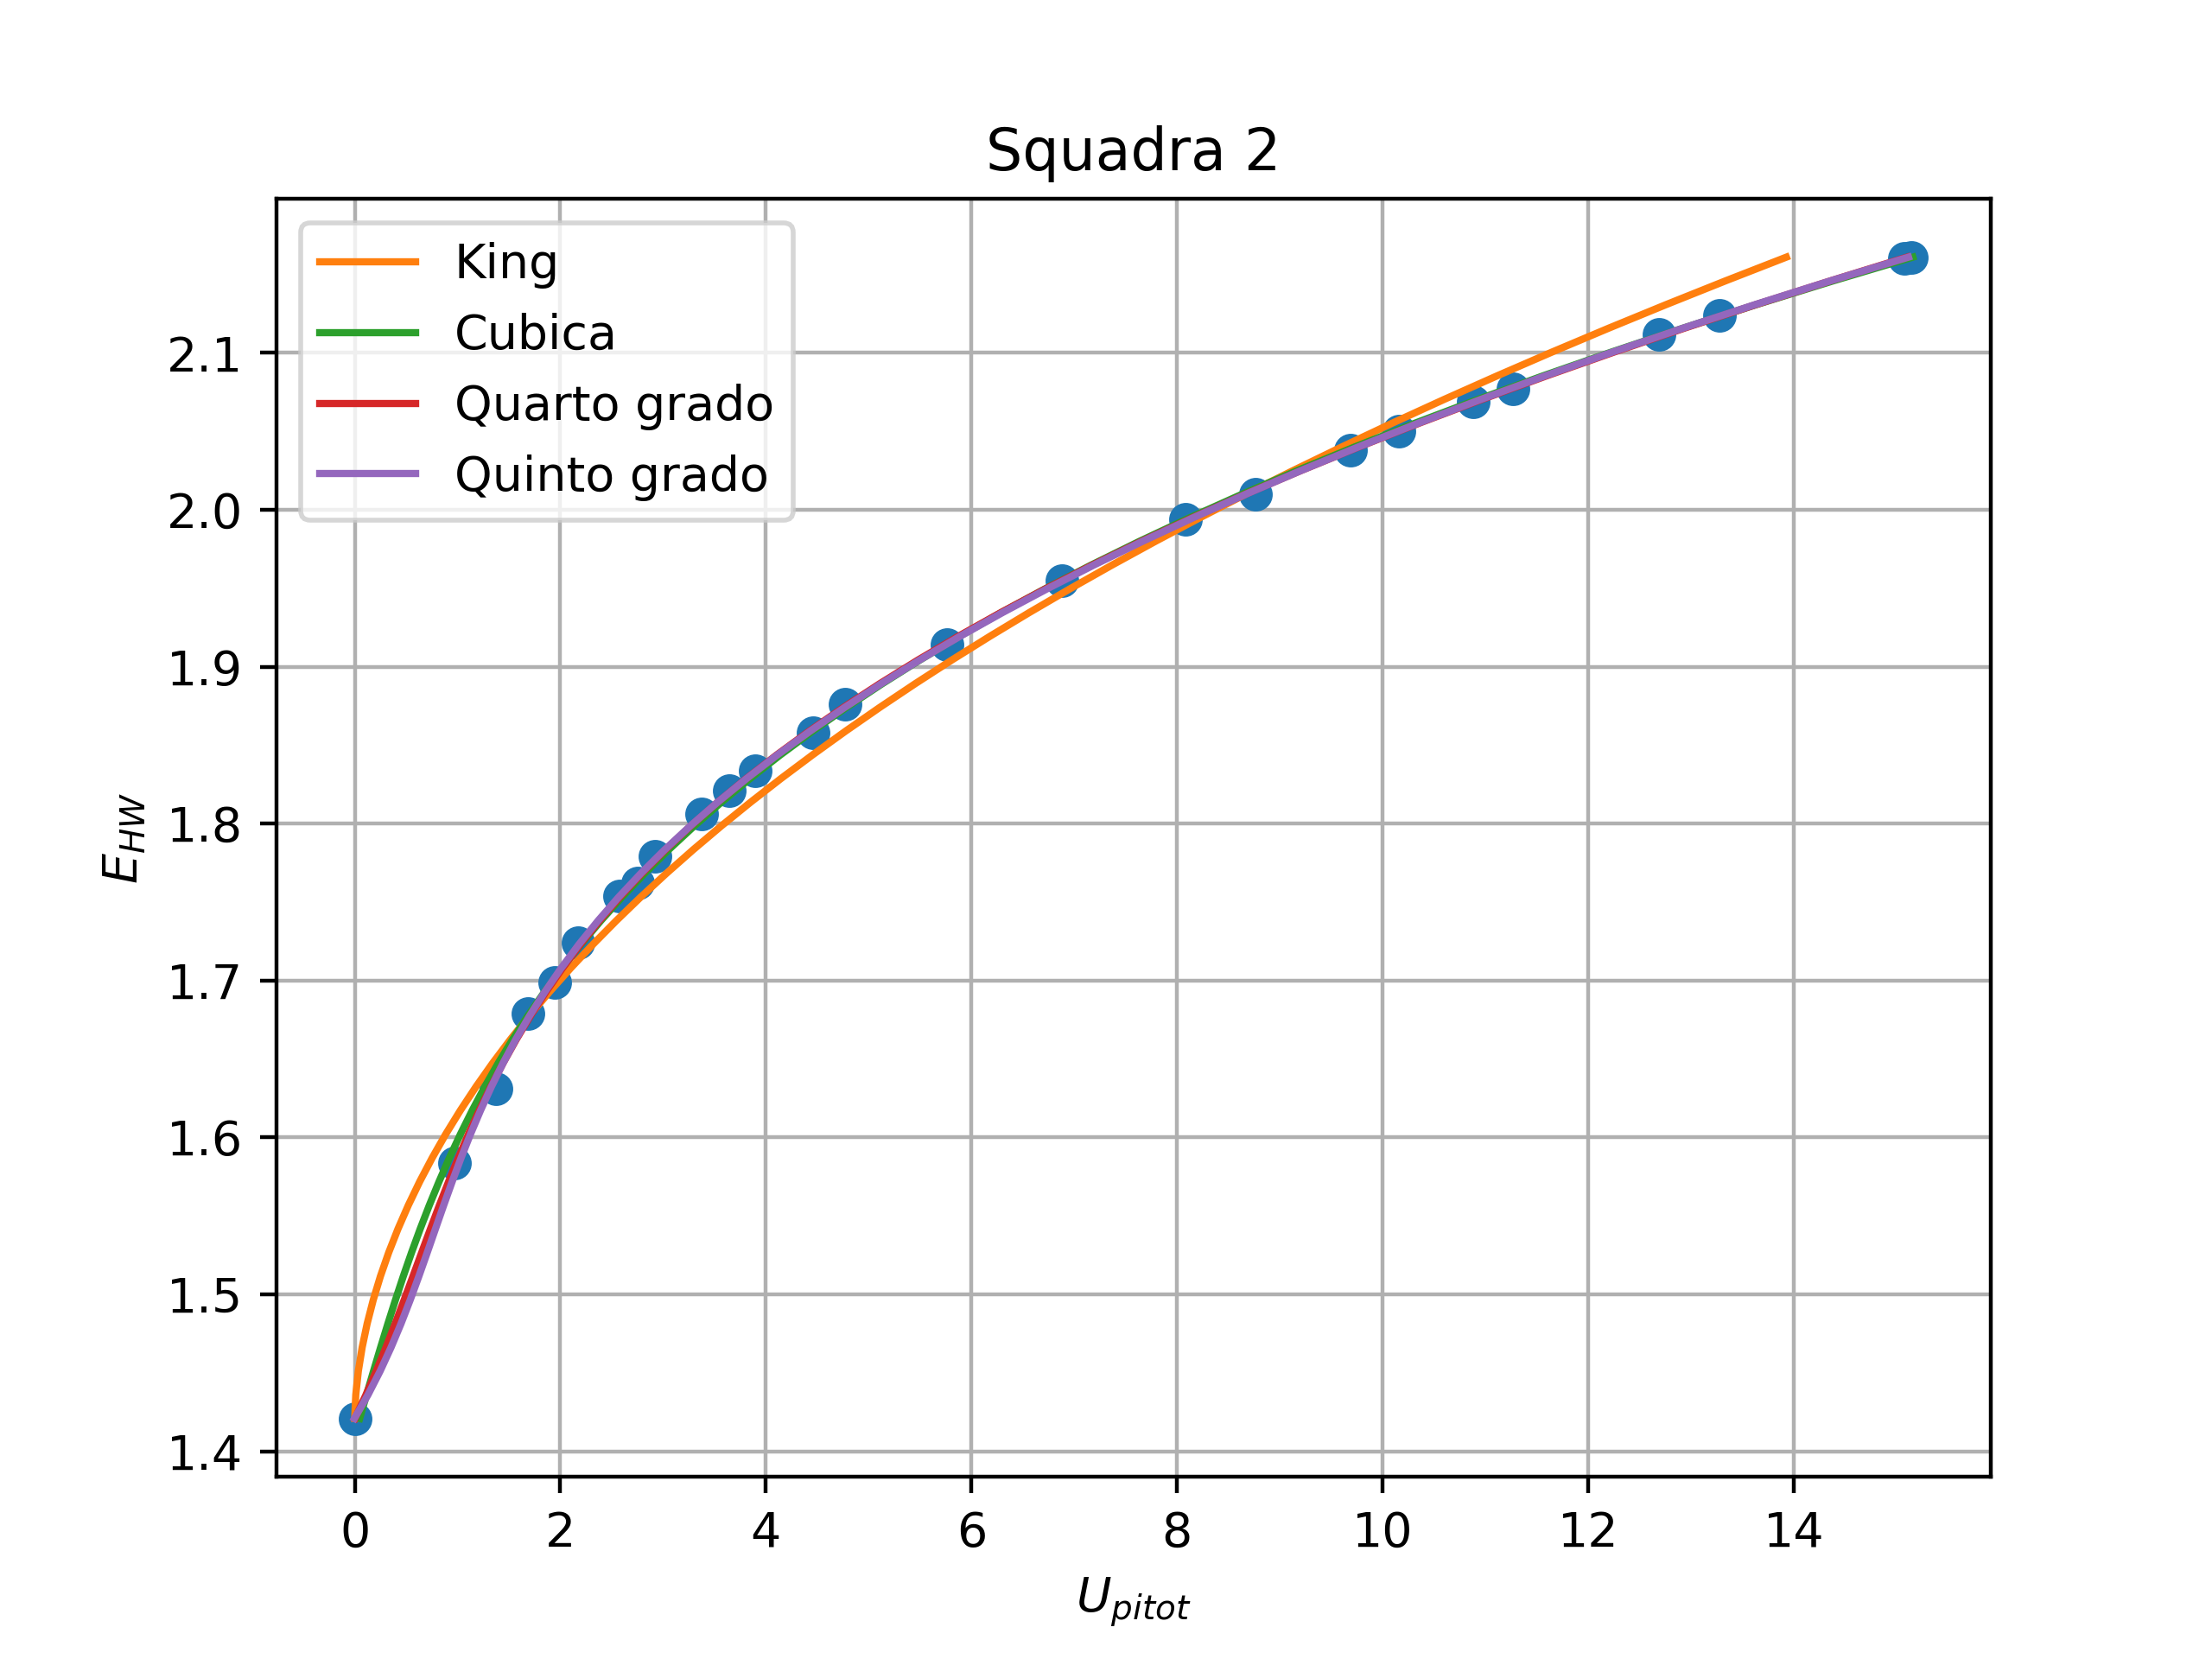
\includegraphics[width=.8\textwidth]{images/8/sq2.png}
    \caption{Squadra 2}
\end{figure}
\begin{figure}[H]
    \centering
    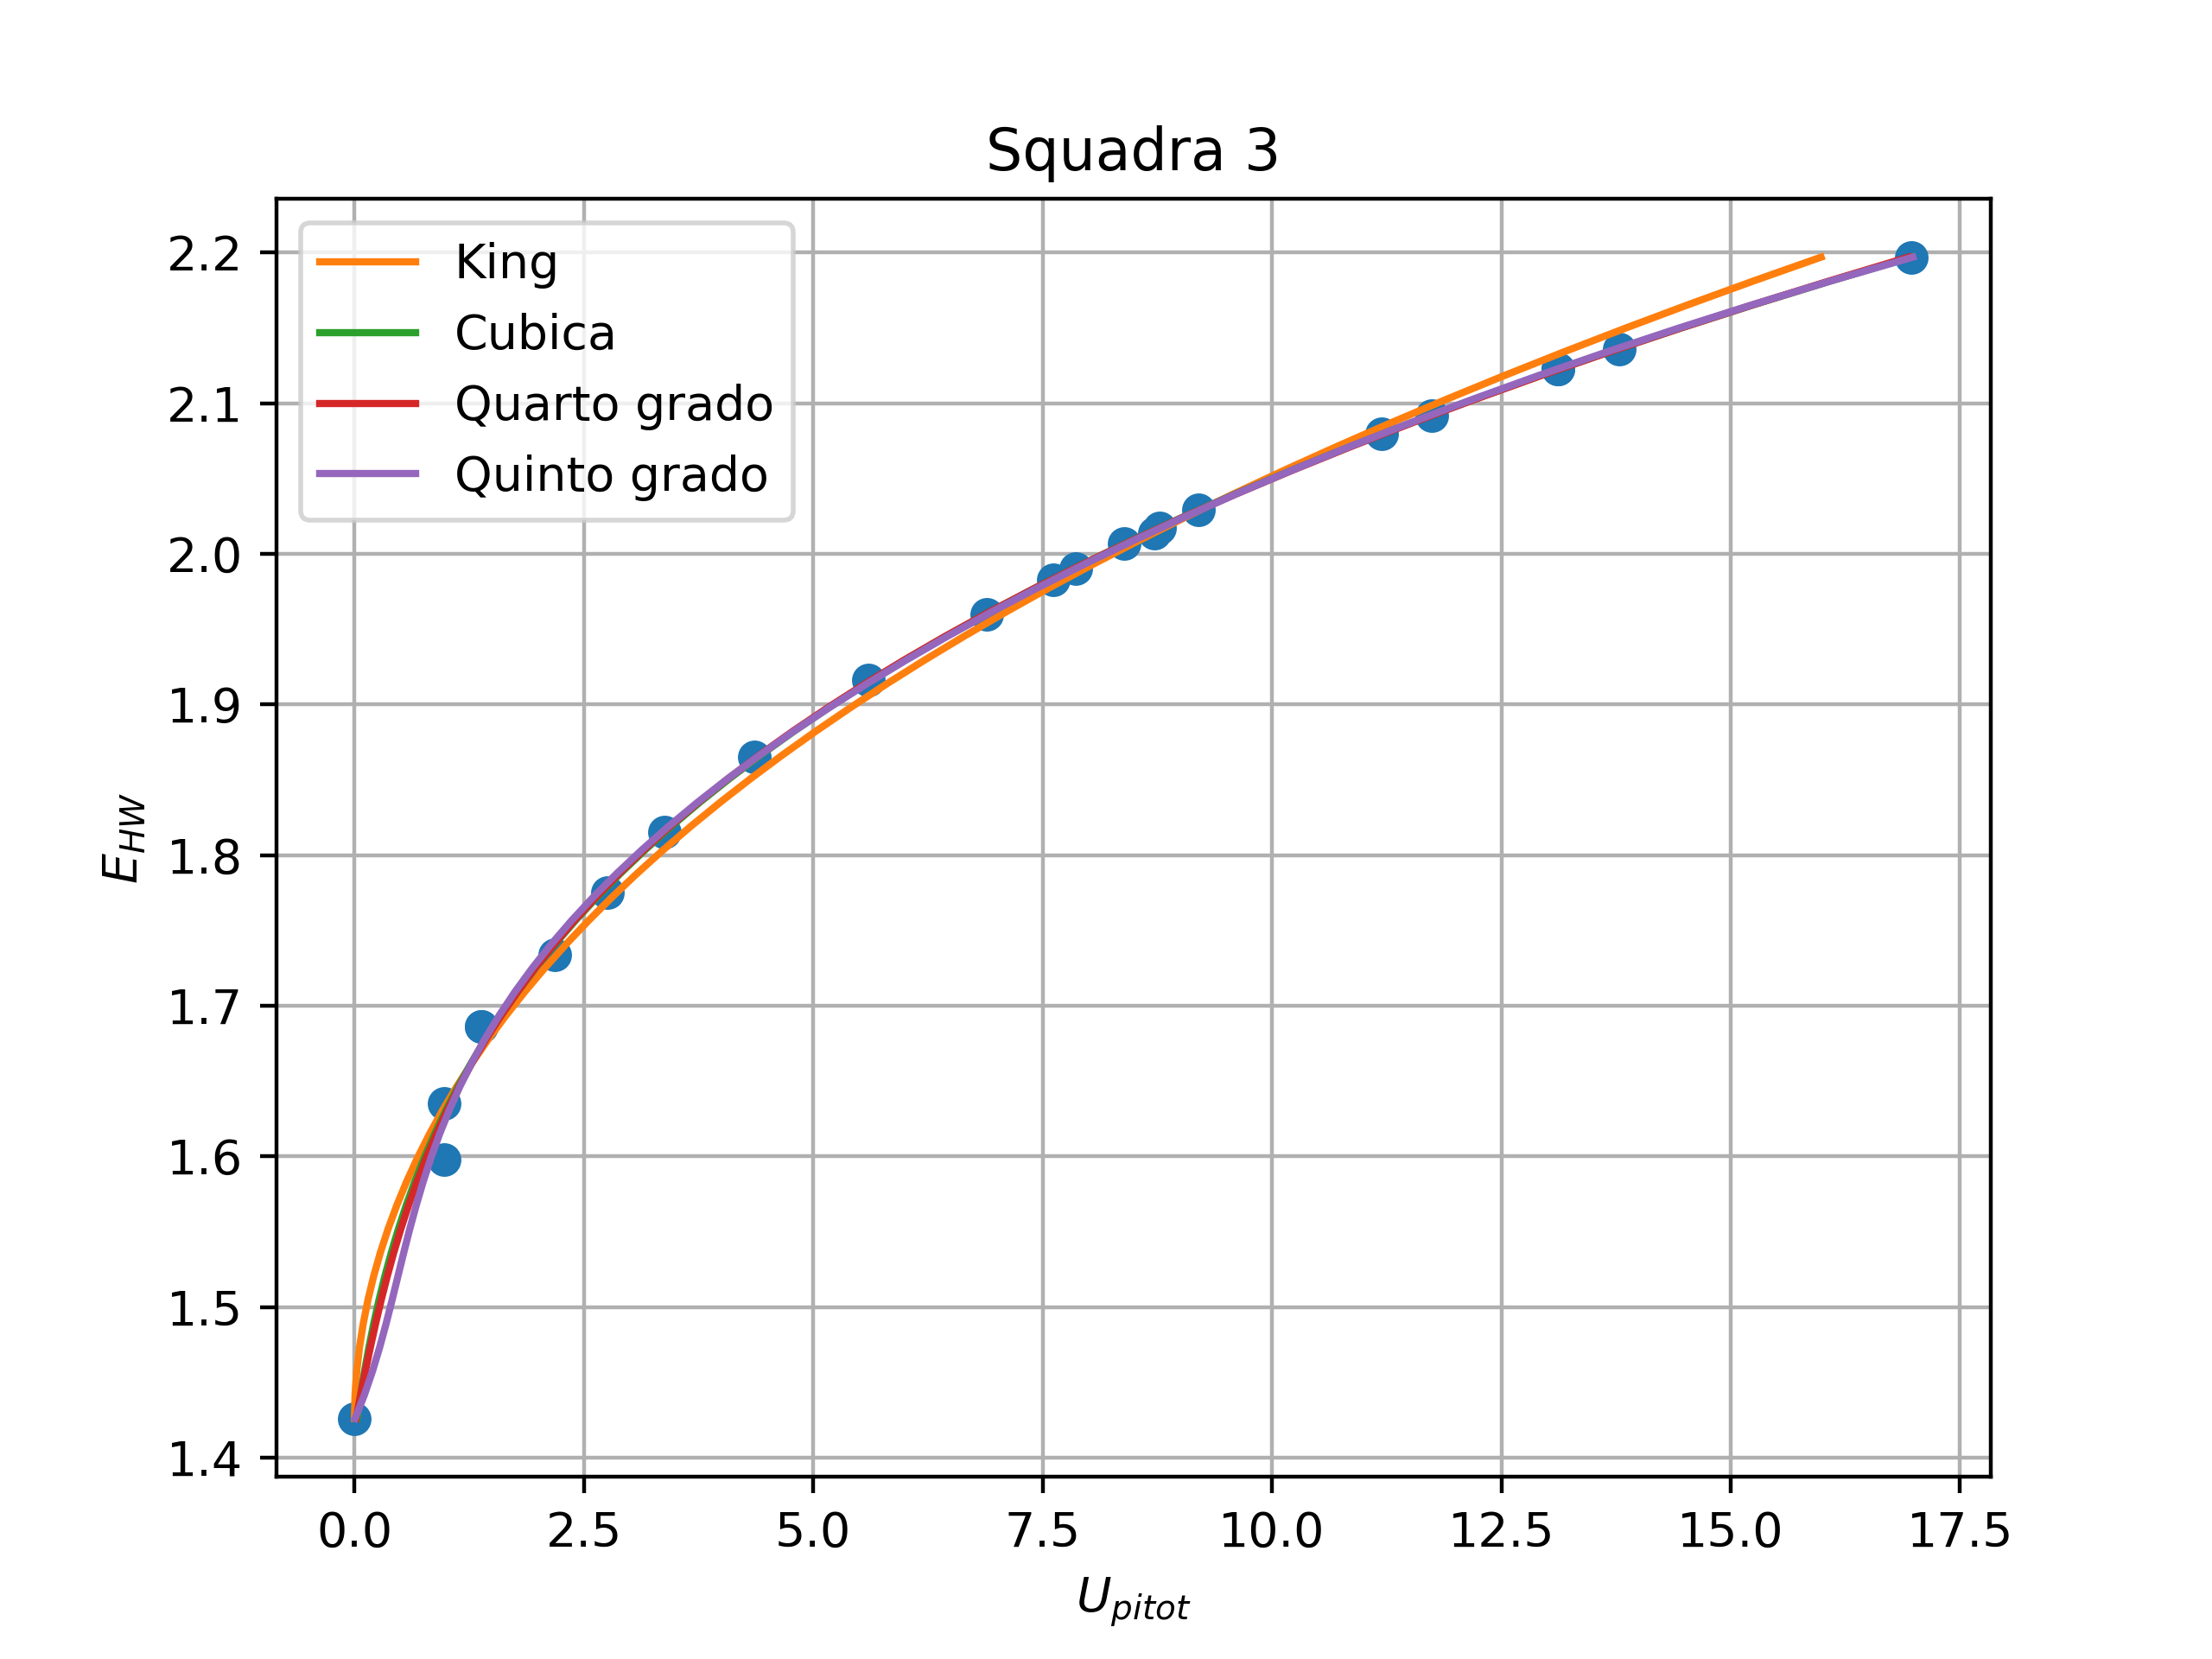
\includegraphics[width=.8\textwidth]{images/8/sq3.png}
    \caption{Squadra 3}
\end{figure}
\begin{figure}[H]
    \centering
    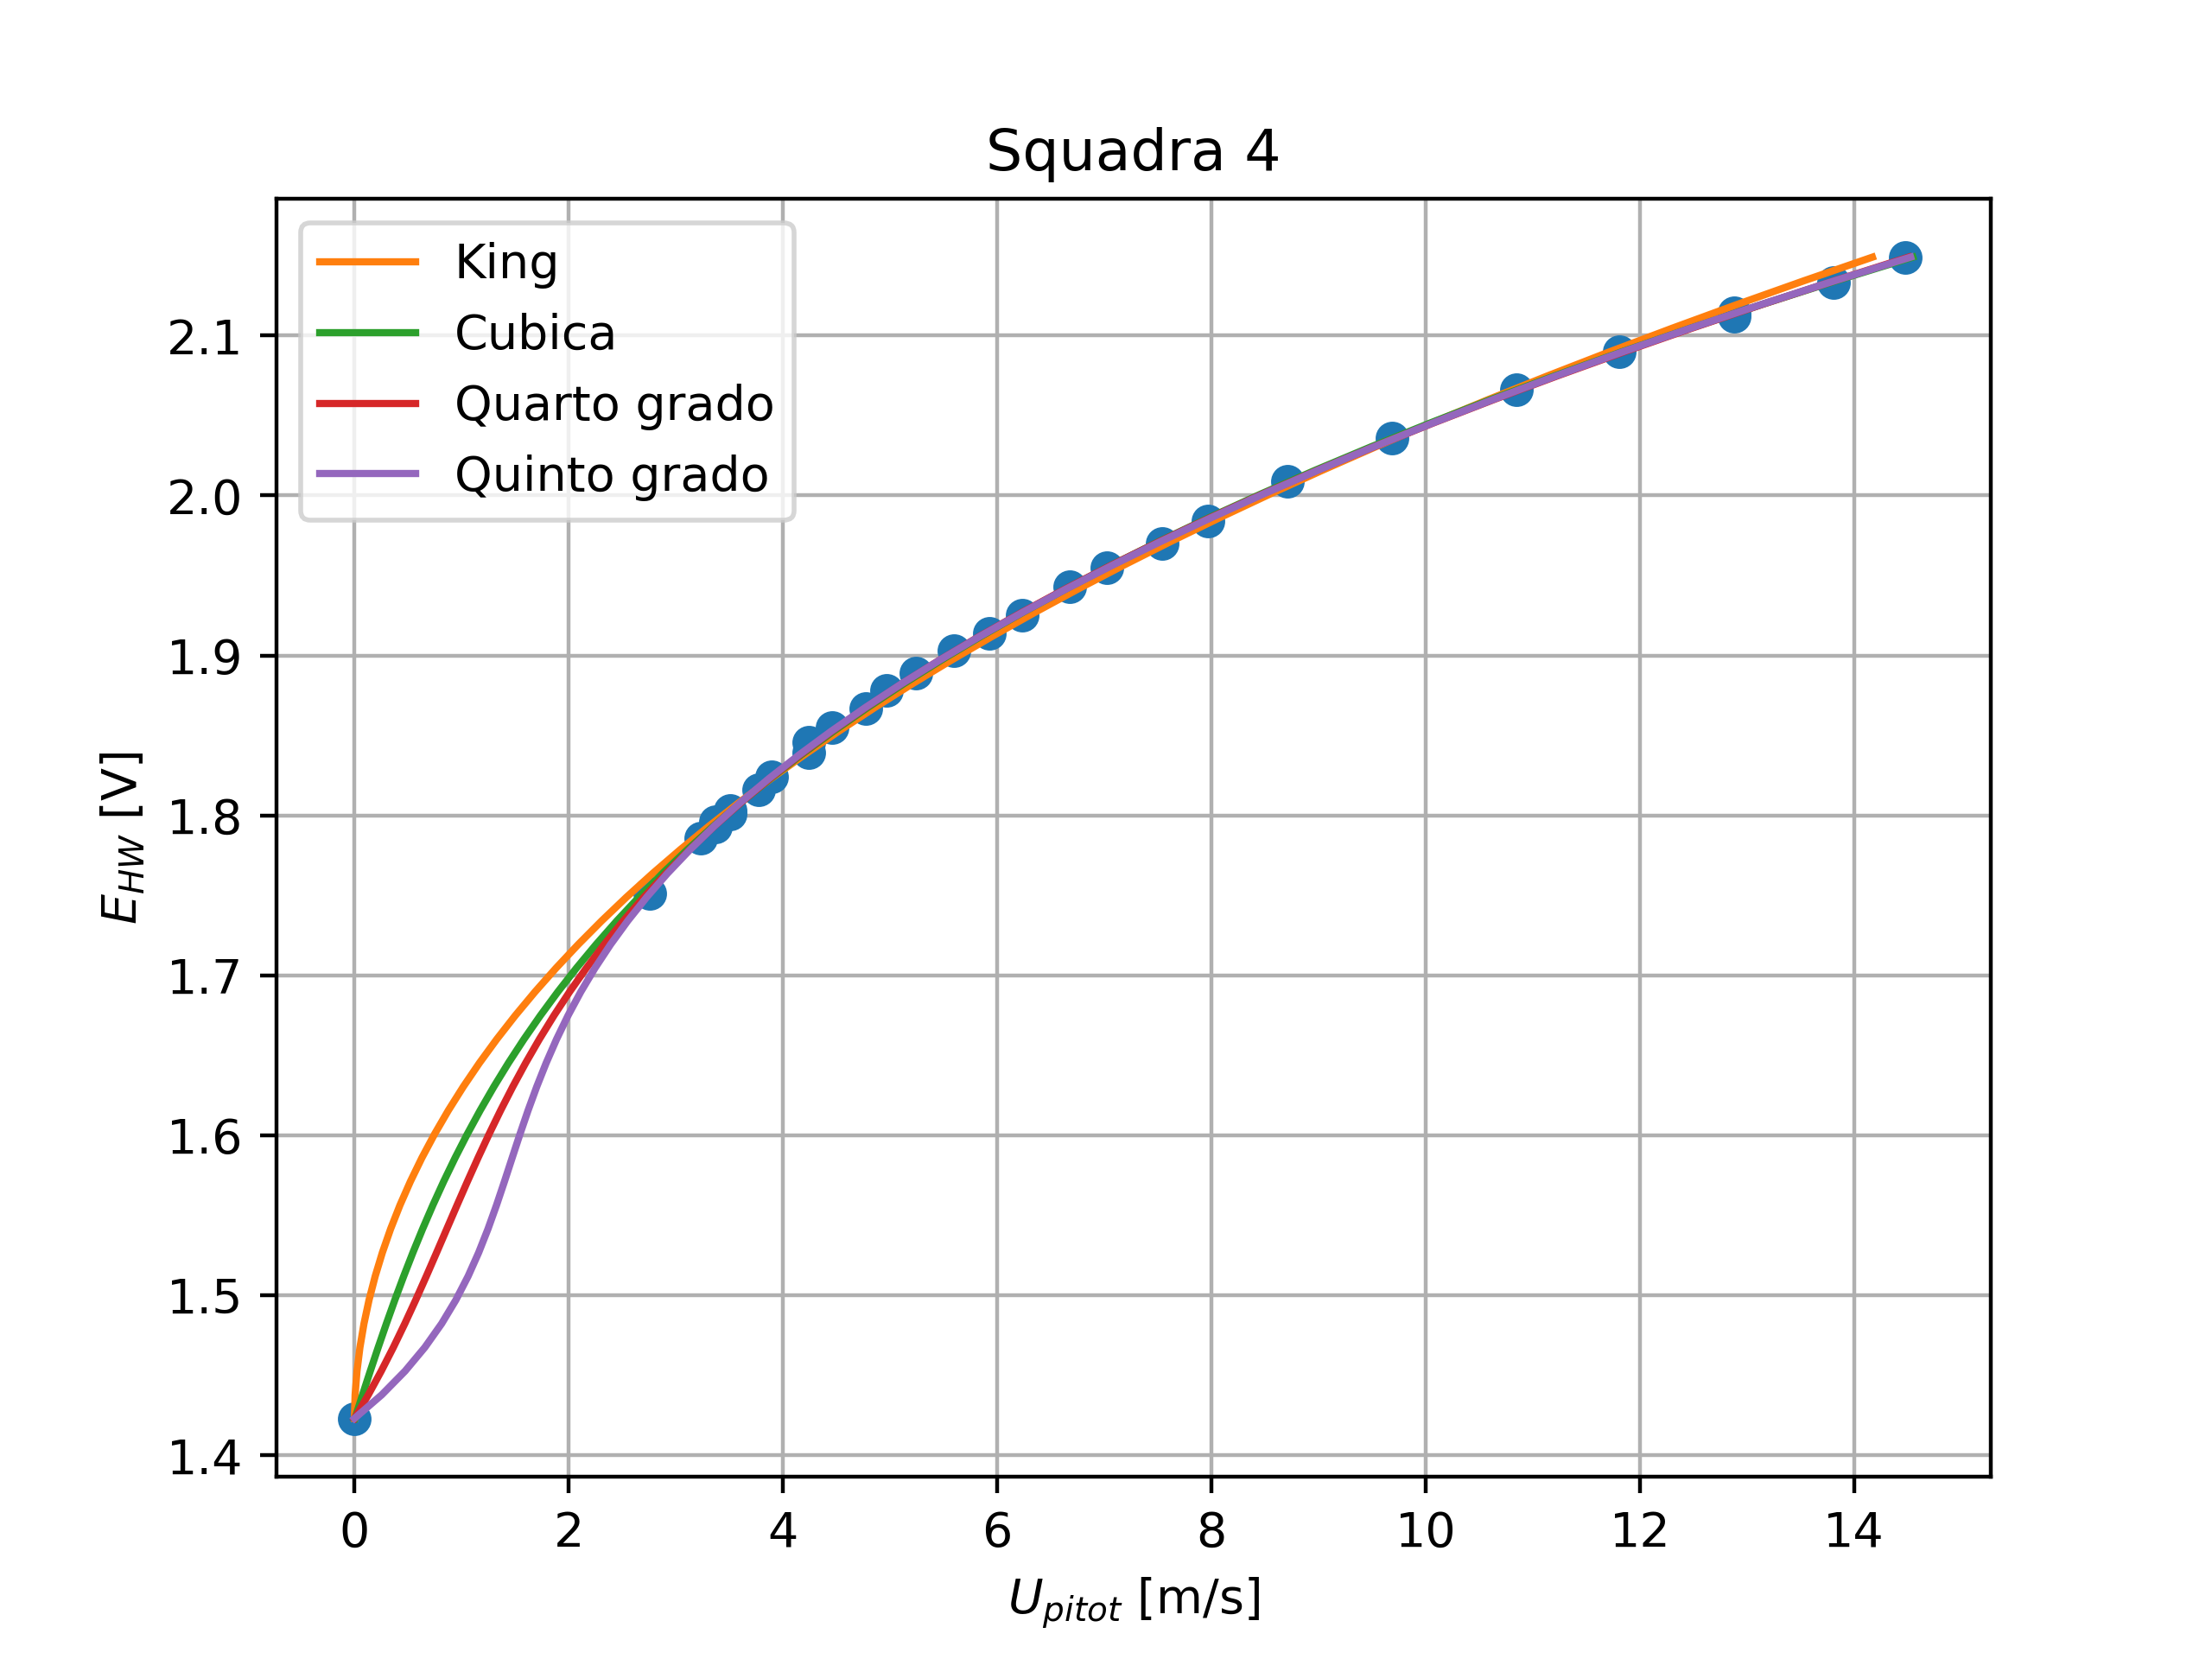
\includegraphics[width=.8\textwidth]{images/8/sq4.png}
    \caption{Squadra 4}
\end{figure}

\noindent Dai risultati ottenuti si osserva come le quattro equazioni di taratura per squadra approssimino molto bene i dati sperimentali.

\newpage
\subsection{Confronto tra le equazioni di taratura}
Per confrontare le equazioni di taratura ottenute, si definisce un parametro $\varepsilon$ che stima la bontà dell'equazione nell'approssimare tutti i punti di taratura:
\begin{equation*}
    \varepsilon = \sqrt{\sum_{i=1}^N\left( \frac{U_{cal}-U_{mis}}{U_{cal}} \right)_i^2}
\end{equation*}
Dove $U_{mis}$ rappresenta il valore di velocità misurato dalla sonda di Pitot e dal trasduttore Setra 239 C, mentre $U_{cal}$ rappresenta il valore di velocità calcolato utilizzando una delle equazioni di taratura.\\\\
Si ottengono i seguenti risultati:
\begin{table}[h]
    \centering
    \begin{tabular}{|c|c|c|c|c|}
    \hline
              & Legge di King & Legge Cubica & Quarto grado & Quinto grado \\ \hline
    Squadra 1 & 0.2492        & 0.1142       & 0.1080       & 0.0817       \\ \hline
    Squadra 2 & 0.4789        & 0.1365       & 0.0664       & 0.0739       \\ \hline
    Squadra 3 & 0.4856        & 0.3282       & 0.3015       & 0.2388       \\ \hline
    Squadra 4 & 0.1120        & 0.0465       & 0.0374       & 0.0358       \\ \hline
    \end{tabular}
\end{table}

\noindent Risulta evidente come le leggi polinomiali approssimino meglio i dati sperimentali con l'aumentare del grado del polinomio. La legge di King, nonostante sia più rapida da ottenere e da utilizzare ha comunque un indice $\varepsilon$ confrontabile con le leggi polinomiali, seppur leggermente maggiore.\\\\
È importante sottolineare come il parametro $\varepsilon$ avvantaggi le leggi polinomiali, infatti fuori dal campo di velocità testato le leggi polinomiali potrebbero avere andamenti completamente non correlati alla realtà, mentre la legge di King, data la sua natura fisica, può ritenersi più affidabile. Questo è evidente dal seguente diagramma, relativo ai dati della quarta squadra:
\begin{figure}[H]
    \centering
    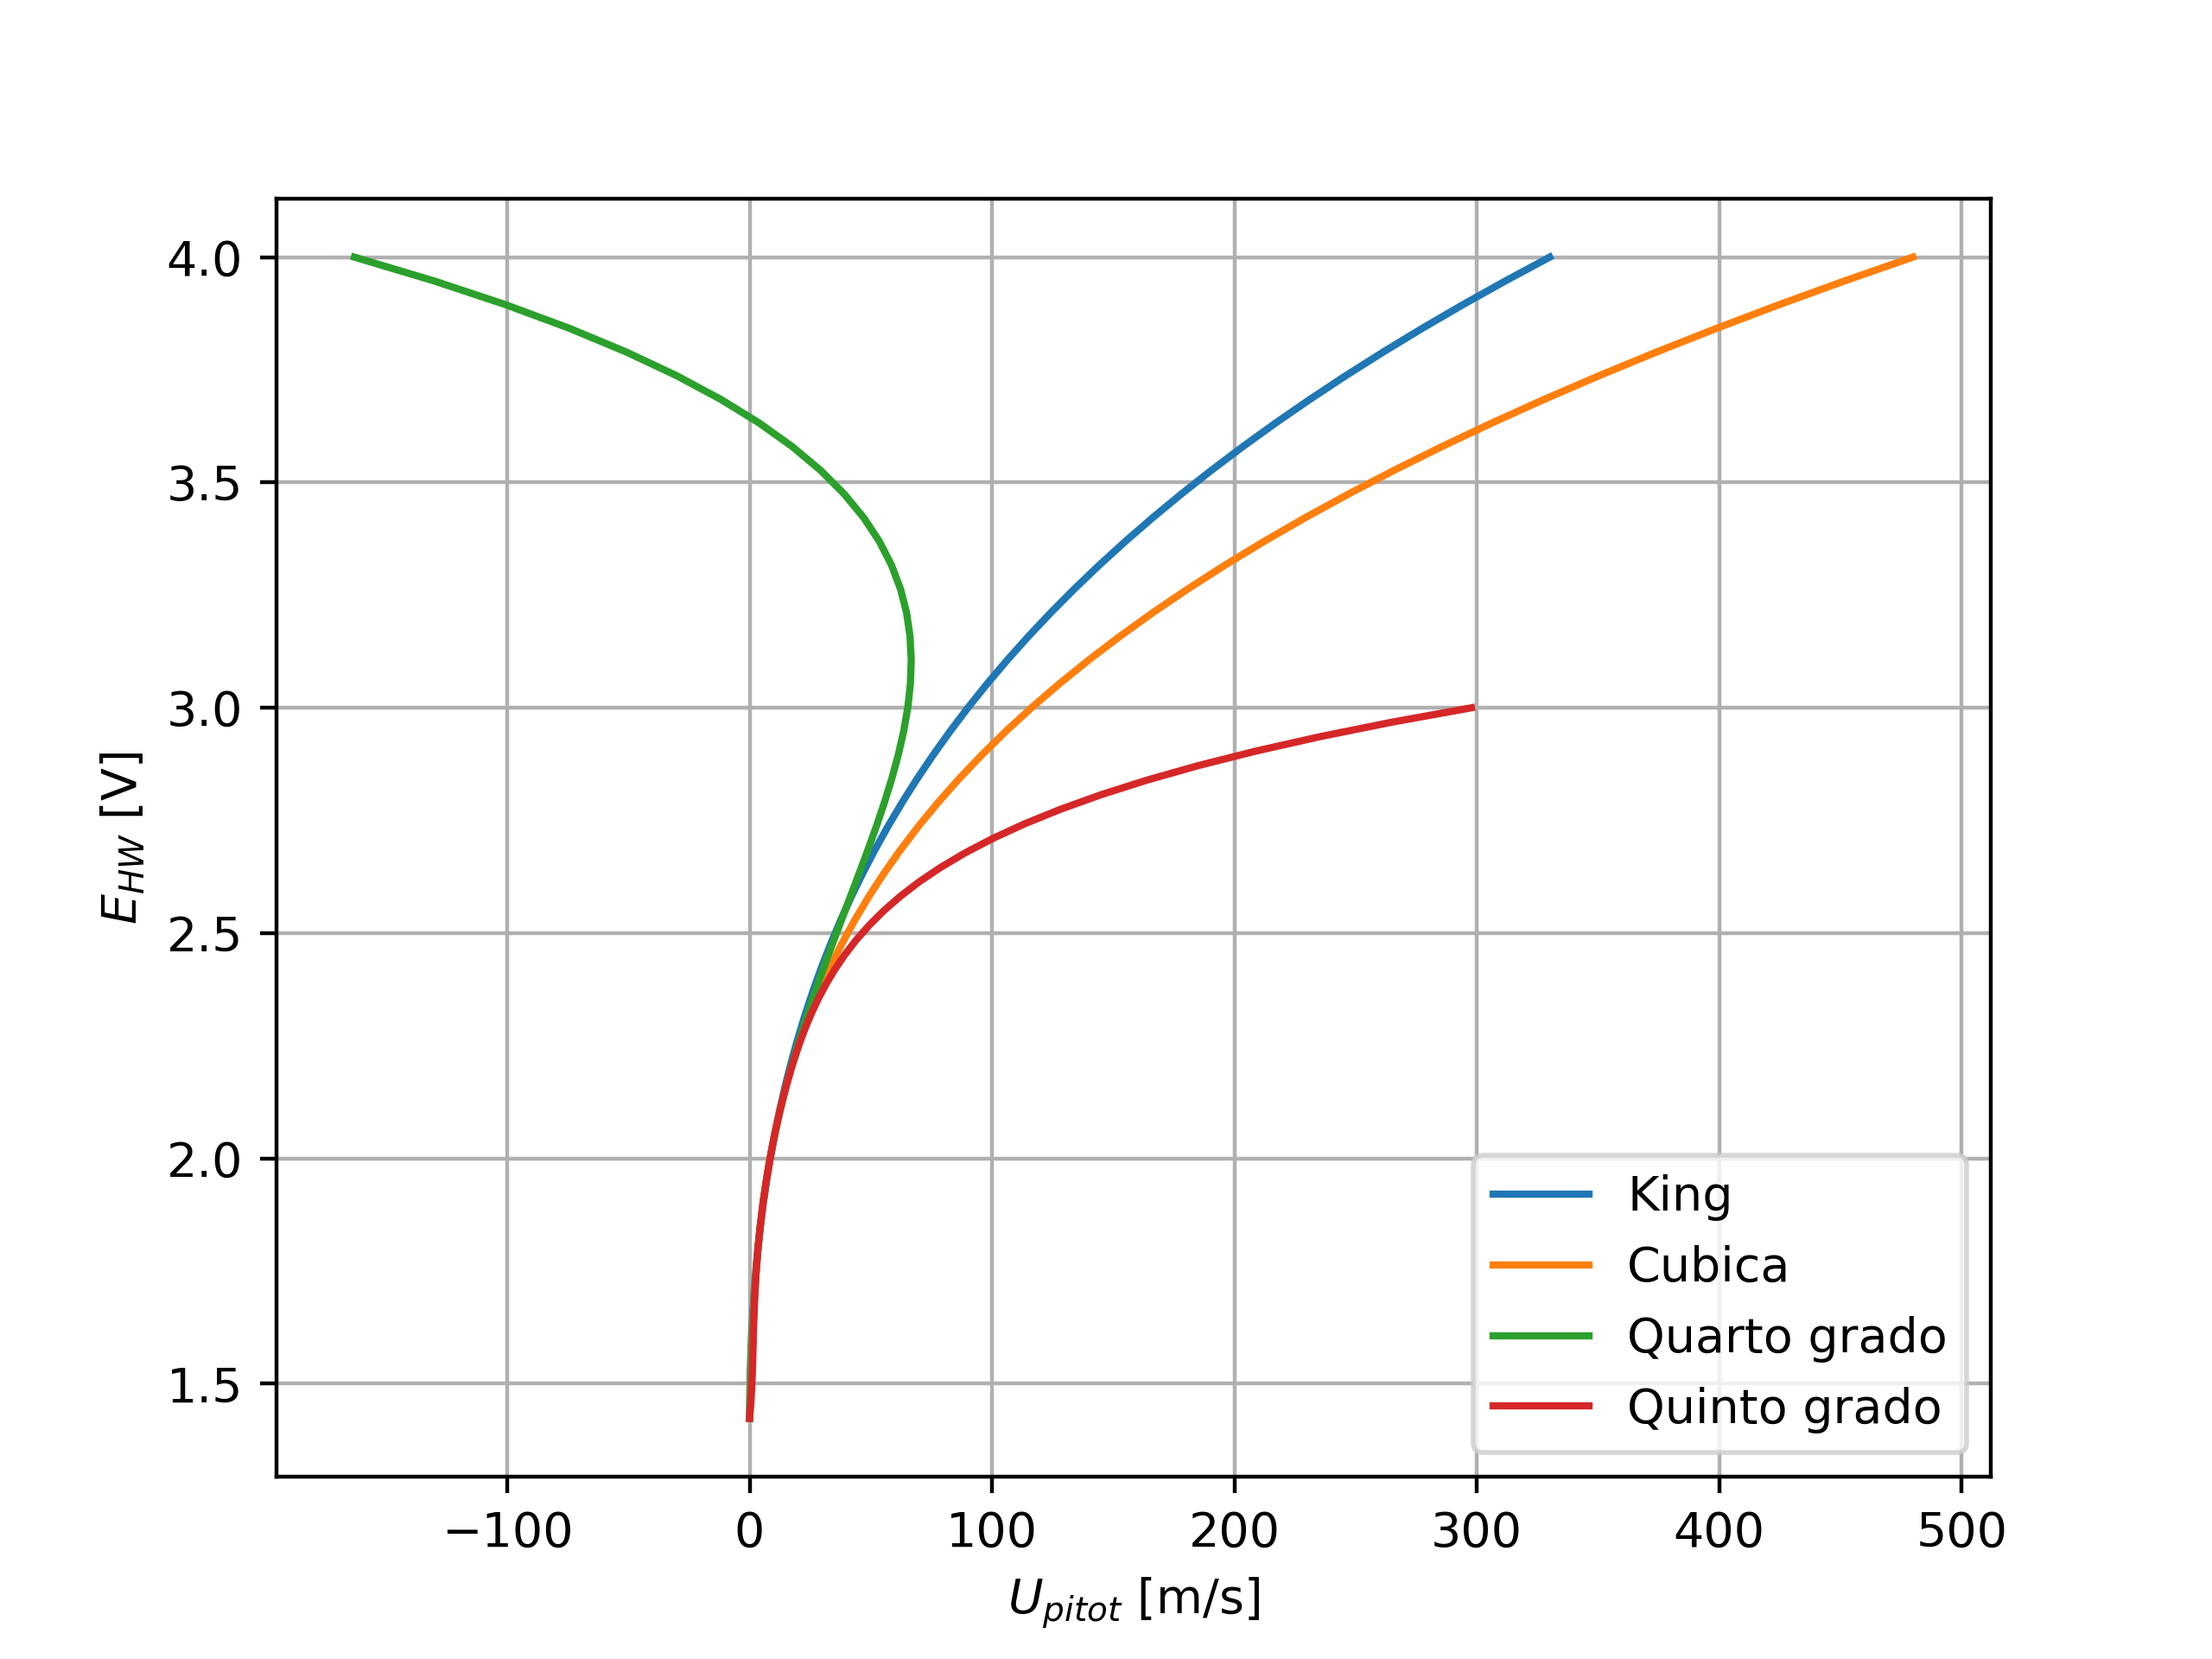
\includegraphics[width=.5\textwidth]{images/8/epswrong.png}
\end{figure}

\noindent È quindi importante assicurarsi di effettuare la taratura della sonda sull'intero campo di velocità sul quale questa deve essere utilizzata.